


\begin{enumerate}
	\item[5.] {Make a graph (simple line plot) of the diabetes percentages for the years 2015 to 2021 (all age groups together). Make a single graph with the four provinces and the national average (indicated as Canada excluding territories) (5 lines). Use different line styles and/or colours for each line plot making sure the national line stands out from the other four. Label the axes clearly and add a title and a legend to your graph.}
	\item[\textbf{Output:}]
	\item[] {\begin{figure}[H]
		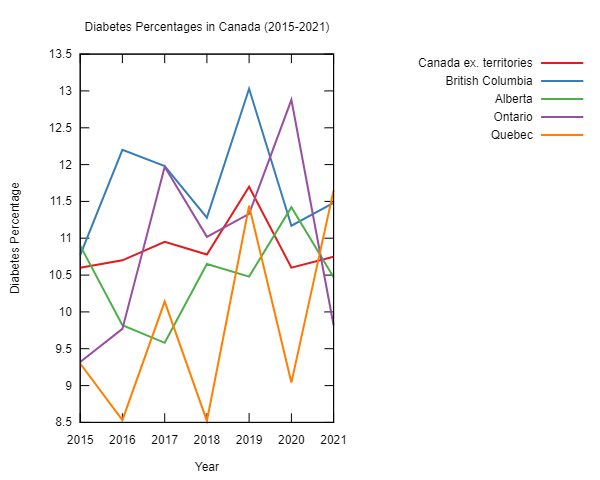
\includegraphics[width=12.75cm]{Q5.png}
		\end{figure}}
	\item[\textbf{Explaination:}]
	\item[] {The line graph produced by this Gnuplot script shows the prevalence rates of diabetes in Canada from 2015 to 2021. The title of the plot accurately explains the goal of the chart, which is to display the prevalence of diabetes in Canada at this time.\\ The years are represented by the x-axis, which has a tick next to each year. The percentage of people who have diabetes is shown on the y-axis.The legend, which is displayed outside the chart on the right side, shows the colour and style of each plotted line.\\ \\ The code makes use of data from a file called "data4a.txt," which contains information on the prevalence rates of diabetes in the four provinces of British Columbia, Alberta, Ontario, and Quebec as well as Canada as a whole. Several line colors and styles are used to represent each province.\\ \\The file's data are plotted with the plot command "data4a.txt. " According to the command "using 1:2," the file's first column should contain the x-axis data (year), and its second should contain the y-axis data (diabetes percentage). The plot command also defines the line style and color for each line in the legend, as well as the title for each line. With the "with lines" option, the plot command links data points with lines.}
	\item[6.] {Make a graph (bar chart) that shows the average percentages of diabetes among the three age groups for the entire country. Label the axes clearly and add a title and a legend to your graph.}
	\item[\textbf{Output:}]
	\item[] {\begin{figure}[H]
		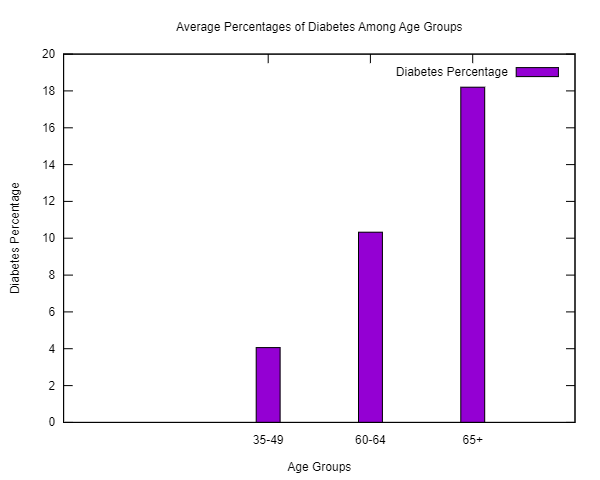
\includegraphics[width=12.75cm]{Q6.png}
		\end{figure}}
	\item[\textbf{Explaination:}]
	\item[] {The graph (bar chart) depicts the average percentages of diabetes across three age groups for the entire country. The three ages  (e.g., "18-34", "35-50", "65 and above").\\ \\ The average prevalence rates of diabetes in various age groups are displayed in a histogram created by this GNUplot. The plot's x-axis displays the age groups, while its y-axis displays the proportion of diabetes cases. The script specifies the width of the histogram bars relative to the available space.\\ \\ In addition, the y-axis range is configured to begin at 0 and terminate at 20, with a 2 unit gap between each y-tick. The height of the relevant bar in the bar chart indicates the prevalence of diabetes in each age group. This bar chart was plotted using a file called” q6.txt”
}
\end{enumerate}

